\documentclass[a4paper]{report}
\usepackage[utf8]{inputenc}
\usepackage[portuguese]{babel}
\usepackage{hyperref}
\usepackage{a4wide}
\hypersetup{pdftitle={3D Map Generation},
pdfauthor={José Ferreira, Jorge Mota},
colorlinks=true,
urlcolor=blue,
linkcolor=black}
\usepackage{subcaption}
\usepackage{listings}
\usepackage{booktabs}
\usepackage{multirow}
\usepackage{appendix}
\usepackage{tikz}
\usepackage{authblk}
\usepackage{bashful}
\usepackage{verbatim}
\usepackage{amssymb}
\usepackage{multirow}
\usepackage{mwe}
\usepackage{float}
\usetikzlibrary{positioning,automata,decorations.markings}

\begin{document}

\title{3D Map Generation}
\author{José Ferreira (A83683), Jorge Mota (A85272)}
\date{\today}

\begin{center}
    \begin{minipage}{0.75\linewidth}
        \centering
        
\includegraphics[width=0.4\textwidth]{images/eng.jpeg}\par\vspace{1cm}
        \vspace{1.5cm}
        \href{https://www.uminho.pt/PT}
        {\color{black}{\scshape\LARGE Universidade do Minho}} \par
        \vspace{1cm}
        \href{https://www.di.uminho.pt/}
        {\color{black}{\scshape\Large Departamento de Informática}} \par
        \vspace{1.5cm}
        \maketitle
    \end{minipage}
\end{center}

\tableofcontents

\pagebreak
\chapter{Introduction}

The aim of this project was to developed a GPU powered procedure using shaders to generate terrain.
To accomplish this we used OpenGL shading language (GLSL) and the Nau3D rendering engine to simplify the usage
of shaders.

%shitiest rendering engine ever Nau3D. 

%is to develop a shader that creates a Terrain. 

% Development

The development of this project began by using a geometry shader to create the points on the terrain. This was
considered a first iteration of our project. However, as we wanted to be able to vary the tessellation value
in run-time, we created a second iteration that uses tessellation shaders to create a the terrain. To increase
the quality of the scene we also added water with an animation that varies overtime. This is our main supported
branch.


\section{Nau Project}

Before going into the project and the implementation itself, we need to leave some notes on the used rendering
engine and how the shaders are loaded and parameterized, this informations will be useful in some explanations.

The \textit{Nau3D} Engine allows the usage of shaders based on the materials instantiation. All materials must
be declared on a XML file with a `\texttt{.mlib}' extension and the rendering context in another XML file with
\texttt{.xml} extension.

In the \texttt{mlib} file the shaders are declared as a material with a \textit{name} that will be called to
be applied to some object

For this project we created two rendering scenarios, for the first iteration and second, and three material
libraries for the first iteration's terrain , and for the second iteration's terrain and water.


\chapter{1st Iteration - Geometry Shader}


In this first iteration we wanted to generate a terrain by a heightmap using a geometry shader, and for that
our rendering pipeline consisted in a \textbf{vertex shader}, a \textbf{geometry shader} and a \textbf{fragment
shader}.

\section{Terrain}

This shaders pipeline is called once per terrain square, generating one individual cell. 
\newline

The \underline{vertex shader} would create a vertex, based on the instance number, having their coordinates
appropriate for indexing the heightmap.

Next, the \underline{geometry shader} receives this created vertex and outputs a triangle strip square, but
the height of each vertex (y axis) of this square was turned into the value of the texture. The normals are
also computed in this step as the gradient of the X and Z axis.

Finally the terrain is colored with the \underline{fragment shader} using a height based pattern for mountains.
\newline

As we progressed, we stared to see some drawbacks on this method, the detail of the terrain was dependant on
the instances number specified by the XML file scene and this limited the tessellation level changing in
runtime, so we started working on a tessellated terrain generation for this purpose.


\begin{figure}[H]
  \centering
  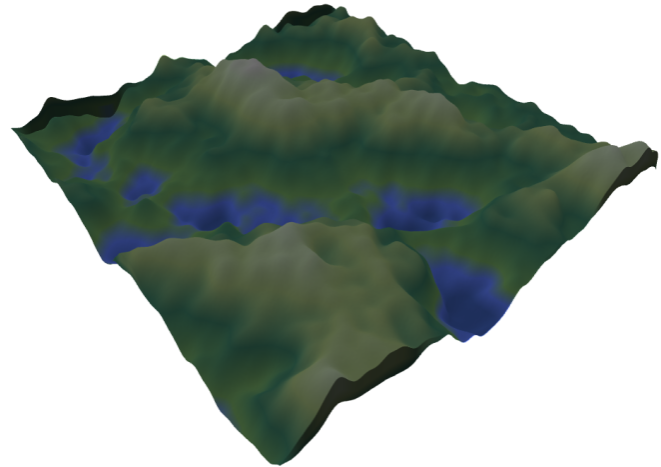
\includegraphics[width=0.6\textwidth]{images/fst_it.png}
  \caption{Terrain generated with geometry shader}
\end{figure}

\chapter{2nd Iteration - Tesselation Shader}

% The vertex shader in this second iteration works as a passthrough of the vertices
% Non-uniform tesselation depending on the distance to the camera

%\section{Tessellation}

Finally, our main implementation followed the same structure as before but we adopted a tessellation
shader (control and evaluation).

To be able to use this tesselation we needed a patched square (or multiples square patches) to
iterate through, and for that we used a \texttt{.patch} file.

%The \underline{vertex shader} in this second iteration works as a pass-through of the vertices


\section{Terrain}

The generation of the terrain consisted in a pipeline with a \textbf{vertex shader}, a \textbf{tesselation control shader}, a \textbf{tesselation evaluation shader} and a \textbf{fragment shader}.

The \underline{vertex shader} in this second iteration works as a pass-through of the patches vertices.

The \underline{tesselation control shader} sets the levels of detail for each patch and the \underline{tesselation evaluation shader} does the work of interpolating the vertices to get the point.

Since the normals are constant during execution time, instead of deriving them like in the first iteration, we use a normals texture to spare this calculations.


%This shader uses the tessellation template developed previously in order to create
the points needed for to create the terrain. 

In this case the height of each point is computed
based on the value present in the texture given by the heightmap. Two parameters were added to control
the main properties of the terrain: scale and width. Altering the scale changes how high the maximum value
is and altering the width changes how large the terrain appears in the final render.

%Some context data is passed from the tessellation shader to the fragment shader
Two values are passed from the tessellation shader to the fragment shader: the \underline{height} of the
point without multiplying by the scale and the \underline{normal} of the point. In the fragment shader this values
are used to calculate the lighting of the point and color. The lighting of the terrain is based on a
directional light declared in the XML project.

\subsection{Color}

To calculate the color of a given point the terrain was divided in two sections, one above water level and
another bellow. What is bellow water goes from a rock-like color towards a sand color as the
point's height gets closer to the water surface. Above water the terrain color goes from a lower forest
color, then forest, lower mountain, middle mountain and mountain top as the point goes towards the
highest point.

Since the color of the terrain depends on the water level, this variable parameter is also an input
from the NAU3D engine.

\section{Skybox}

As a detail of the scene we decided to apply a skybox in the scene to be able to blend the terrain, and
produce reflections in the water. For this step we got a set of images for the sky and used a cube model
to place in the scene. 

The model already specifies the path to the textures so the only mechanics needed was the rendering of
this model, and for this we made a very simple vertex and fragment shaders combination to process the vertices
and place the texture color, no light is applied.

\begin{figure}[H]
  \centering
  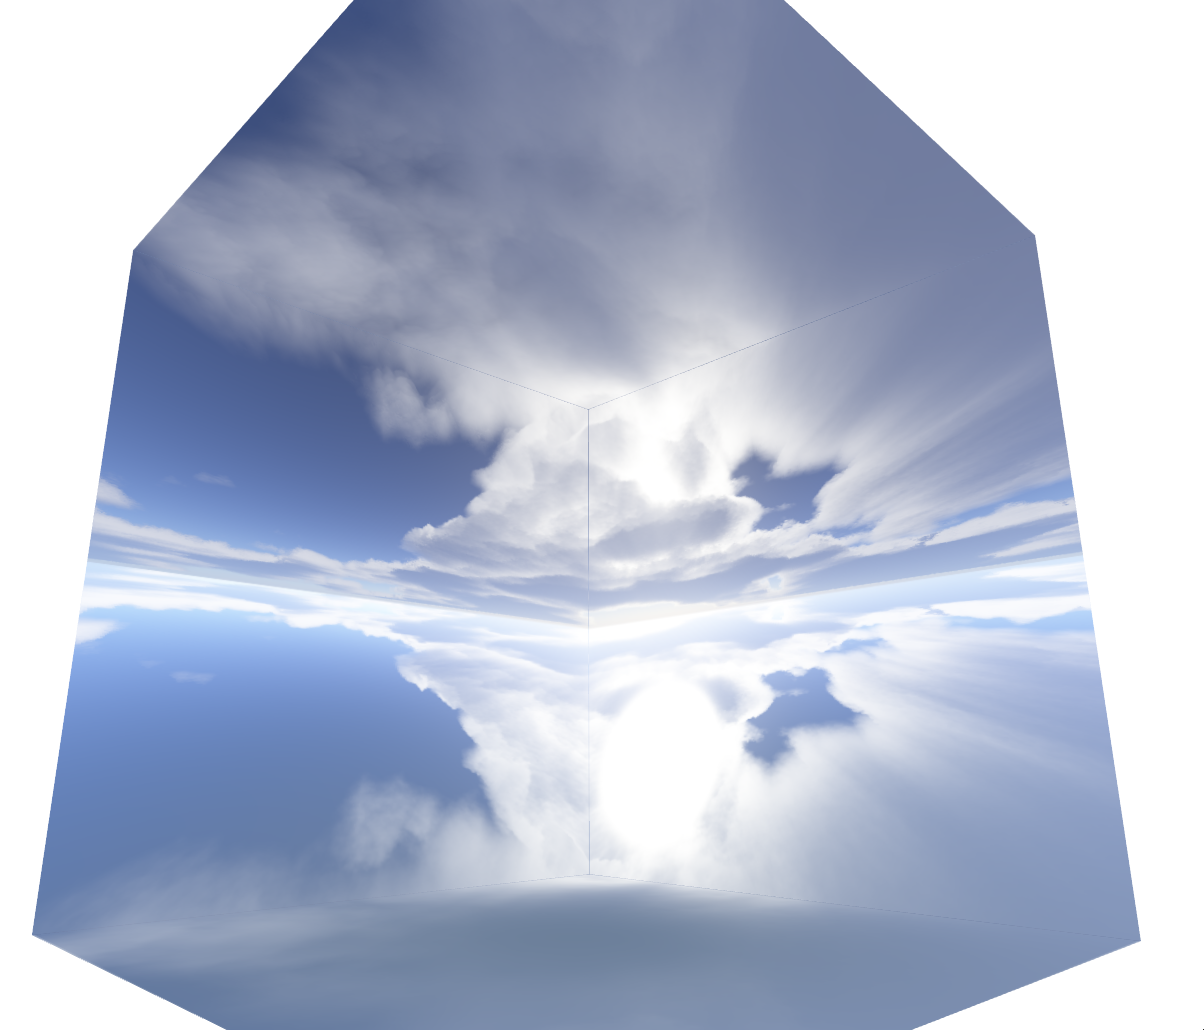
\includegraphics[width=0.8\textwidth]{images/skybox.png}
  \caption{skybox}
\end{figure}


\section{Water}

To add realism to the final terrain and create a better final result, water with an animation was added.
The tessellation shader is almost the same as the one used for the terrain with the only difference being on
how the height of the point is calculated. Instead of using the value of a pre-calculated texture a
mathematical formula using sums of sin is used. To change the properties of the wave frequency and height
can be changed externally. In the following formula the position of the point is (px, pz), t is time in
seconds after the program has started, wf is wave frequency and wh is wave height.

\[  sin((px + pz - 1) * wf + t) * wh \]
\[ + sin((pz - 1) * wf * 2 + t * 2) * wh / 10 \]
\[ + sin((px - 1) * wf * 1.5 + t  * 2) * wh / 5  + wl \]

Then the water tessellation shader gets the value in the terrain texture and passes to the fragment shader
the terrain height and the water height.

Using this values, in the fragment shader, a variable foam cutoff is used to create \textbf{foam} where the water
is near the coast line. The algorithm compares the water height and the terrain height and if it bellow a given
threshold it mixes the water color with the foam color until it is only foam color when the water intersects the
terrain.

\subsection{Cube Mapping}

In order to provide an illusion of reflection of the skybox, surface cubemapping was implemented in the
water fragment shader. To achieve this we computed the reflection vector of the camera direction and the
normal and used the result vector coordinates to sample the \texttt{samplerCube} unit provided as argument.

\begin{figure}[H]
  \centering
  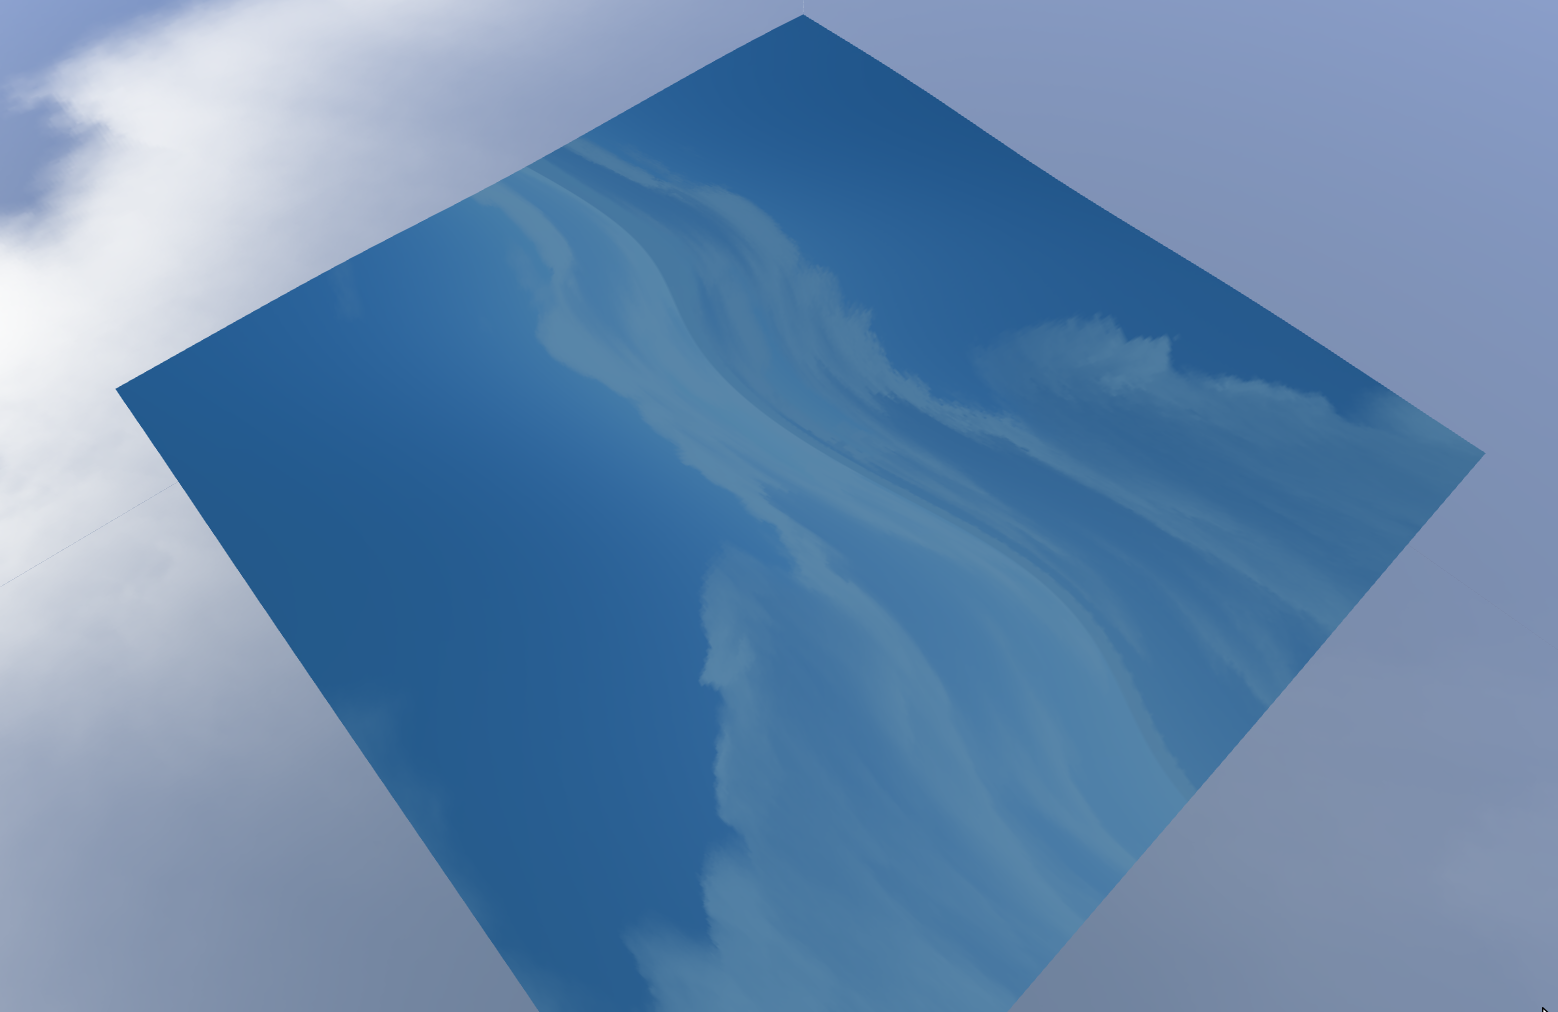
\includegraphics[width=0.8\textwidth]{images/water_reflection.png}
  \caption{water reflecting the sky}
\end{figure}

\chapter{Final Result}

\begin{figure}[H]
  \centering
  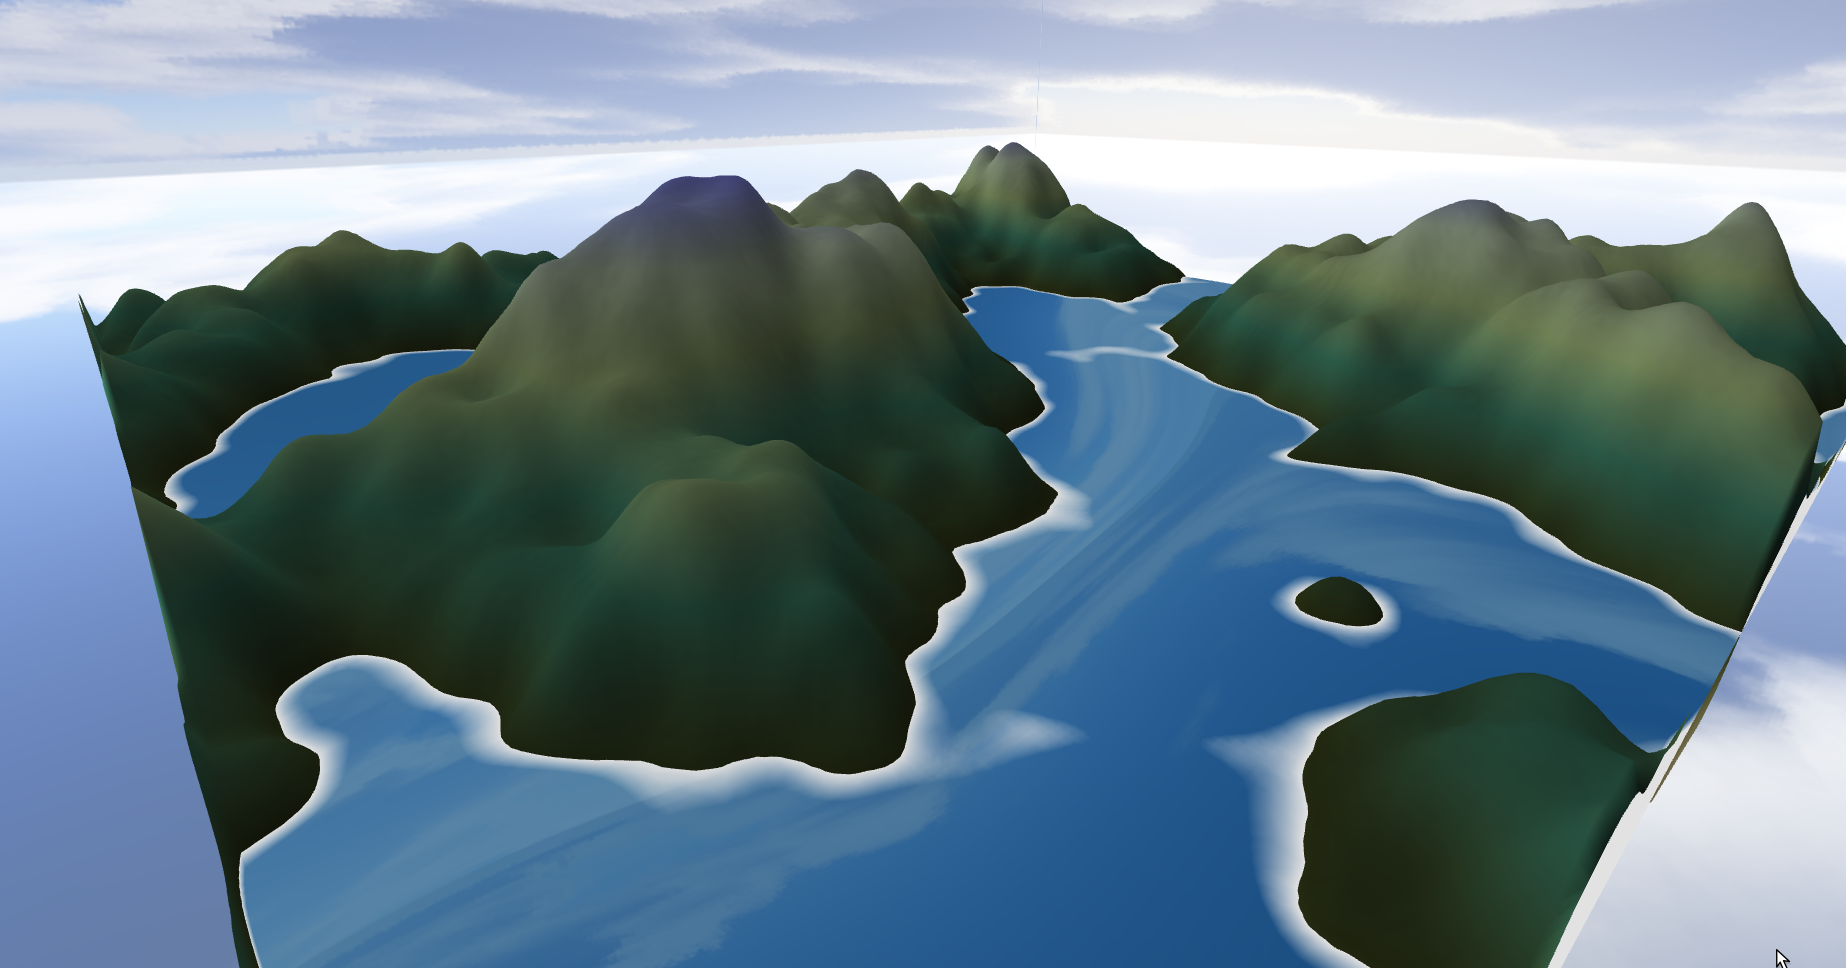
\includegraphics[width=\textwidth]{images/results1.png}
  \caption{outside of the terrain}
\end{figure}

\begin{figure}[H]
  \centering
  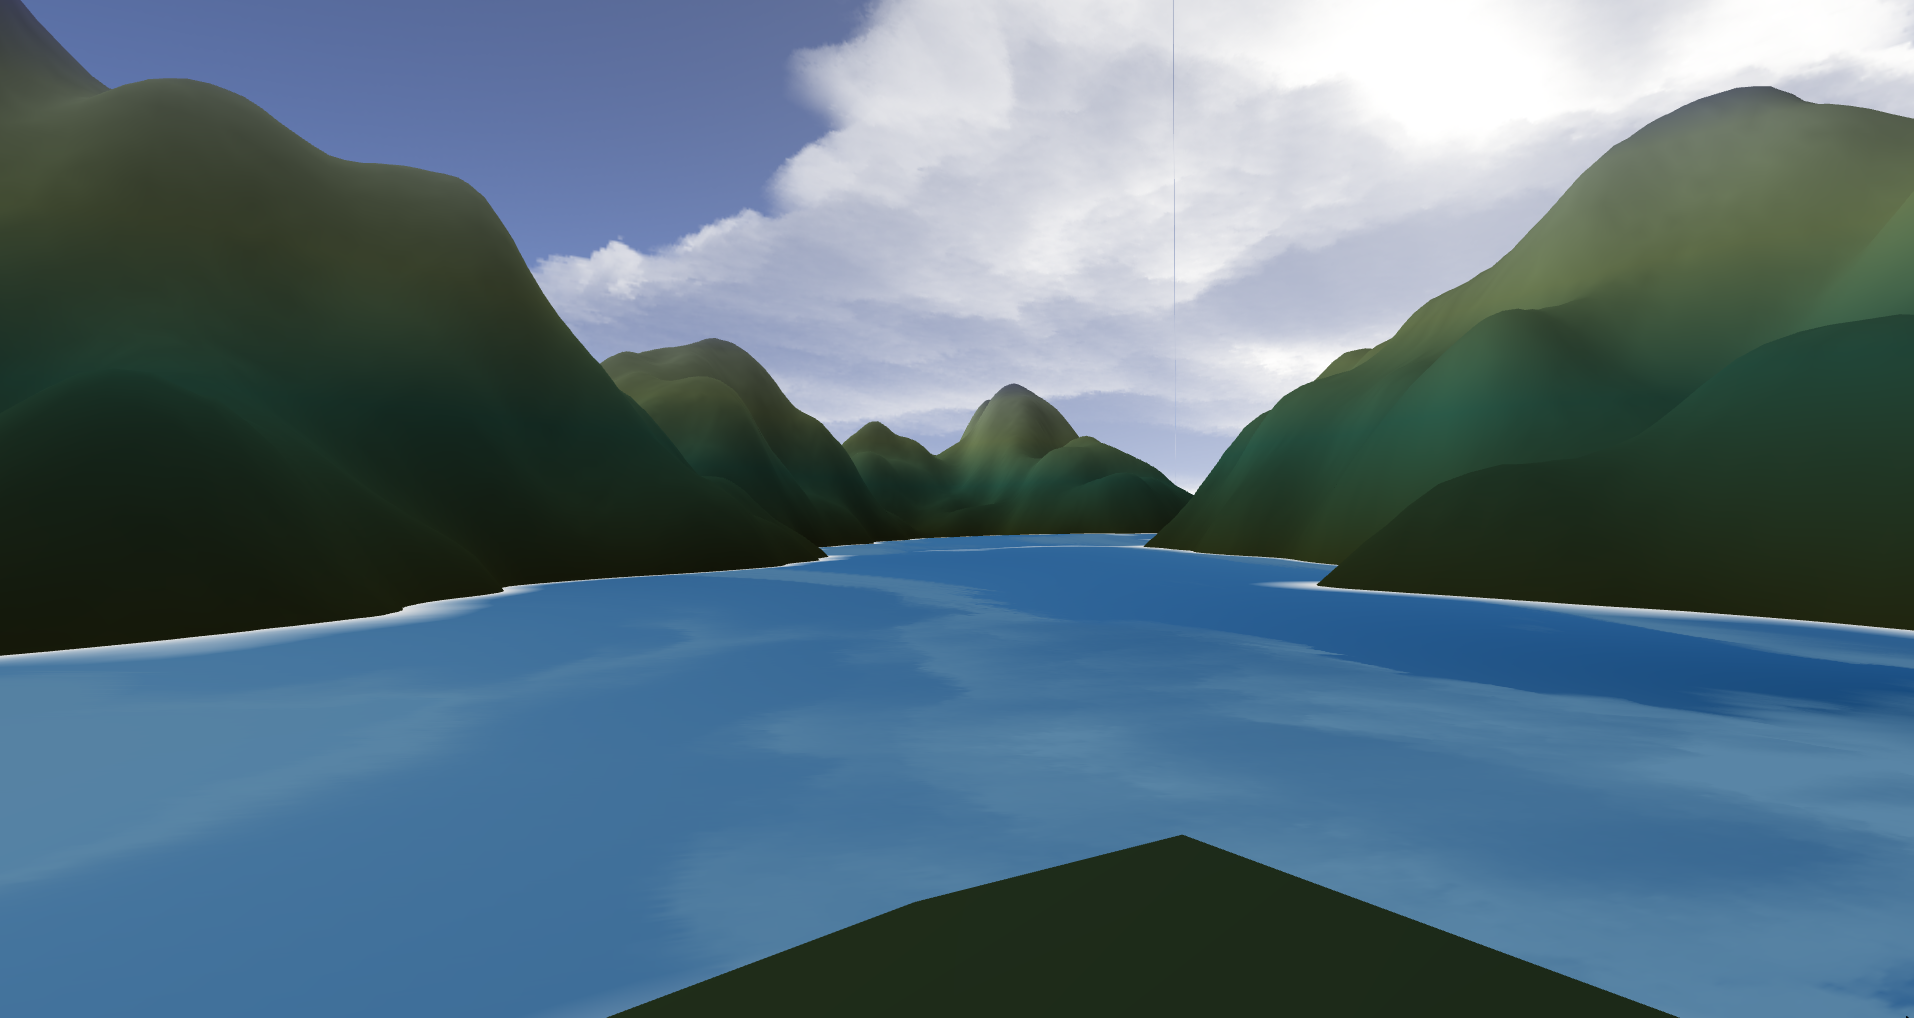
\includegraphics[width=\textwidth]{images/results2.png}
  \caption{above water}
\end{figure}

\begin{figure}[H]
  \centering
  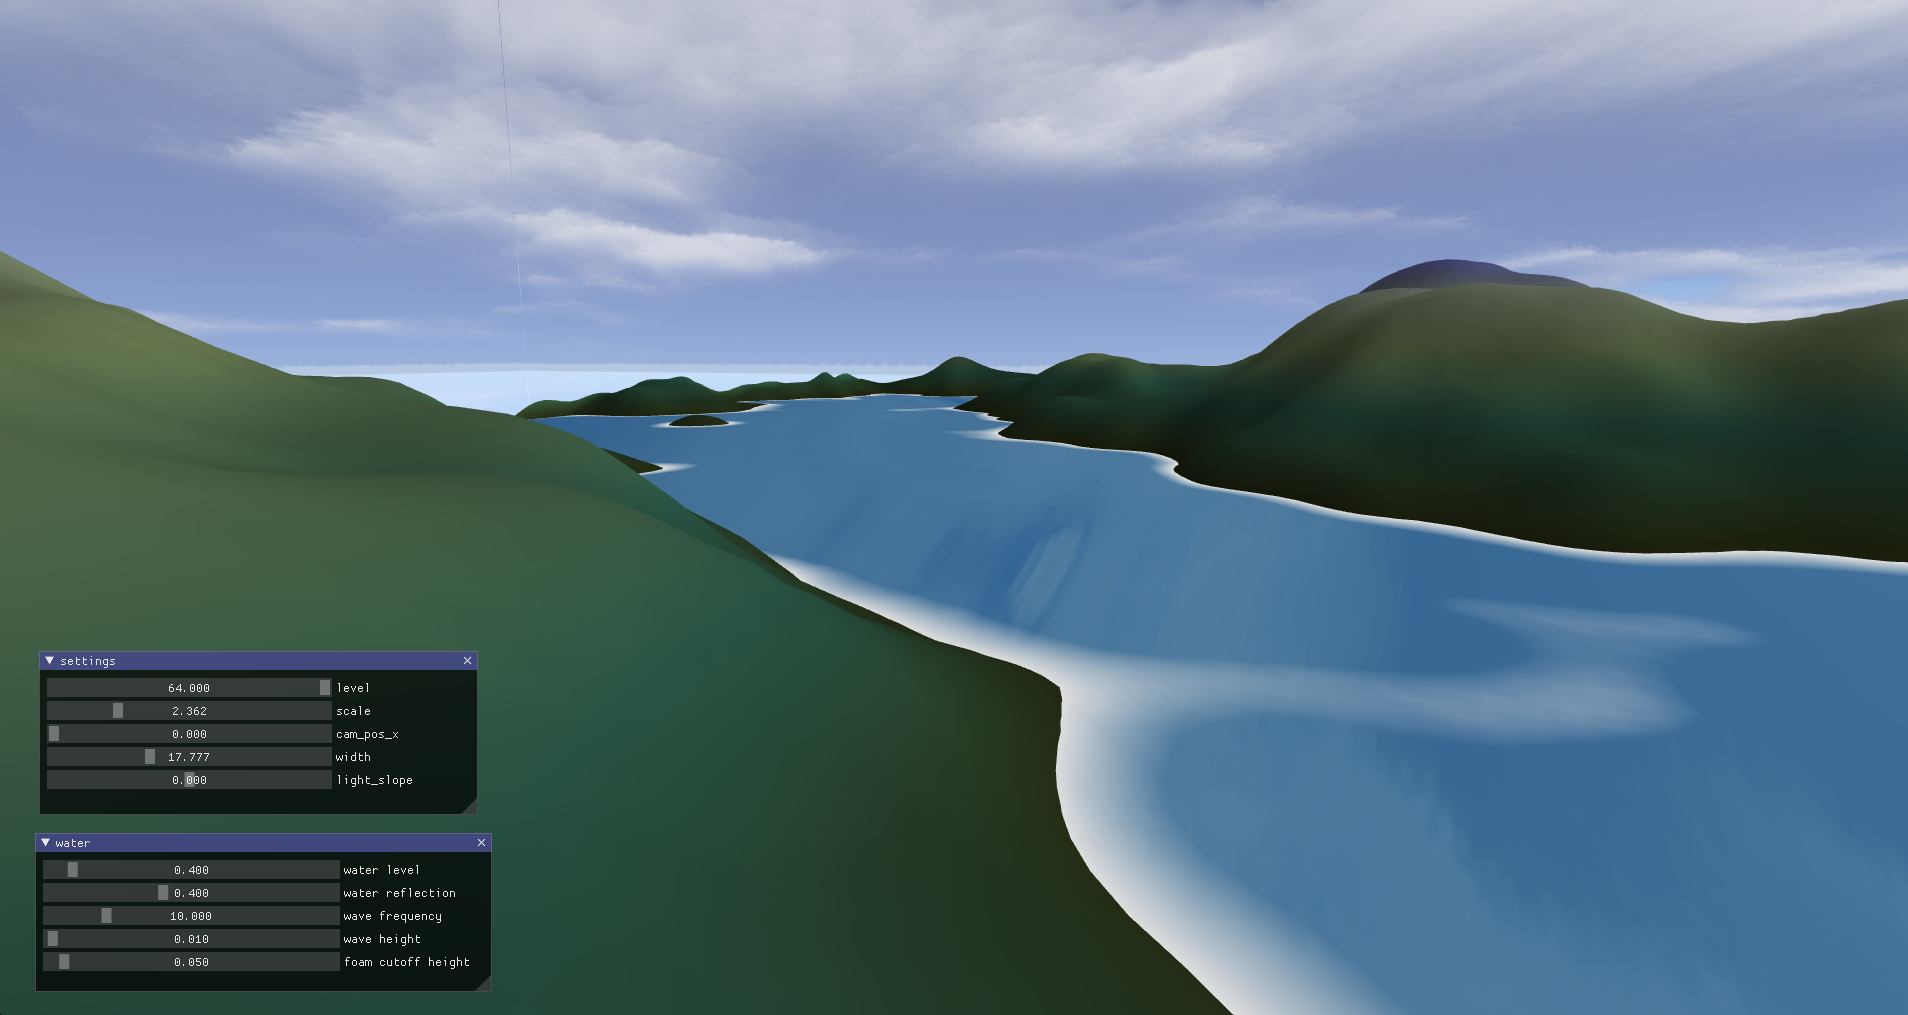
\includegraphics[width=\textwidth]{images/results3.png}
  \caption{NAU3D interface}
\end{figure}

\chapter{Conclusion and Future work}
Concluding, with this work we developed a set of shaders that when combined can create a terrain with a pleasing minimalist aesthetic. In this work we implemented relevant shader related topics covered in classes.

As future work we would like to improve some areas of our work, mainly finish the implementation of non-uniform level tessellation based on distance to camera (we had some problems in the blending of the different levels of tesselation in between patches) and improve the performance of the height map generator. 

We also made some progress in hydraulic erosion with the use compute shaders but with some issues occurring and the time constraining didn't allow us to finish on time, although we could simulate rain droplets iterations.

\begin{figure}[H]
  \centering
  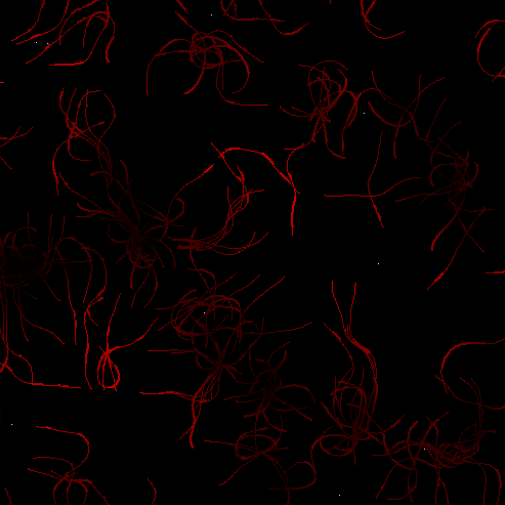
\includegraphics[width=0.3\textwidth]{images/droplets.png}
  \caption{Hydrolic Erosion droplets iteration progress}
\end{figure}

Finally we would like to add procedurelly generated grass, bushes and trees that react to wind direction in order to create a more complete and immersive terrain.



%\chapter{References}

\end{document}